% Provenance (never printed): cycle 2 "Questionner le monde" (states of water in
% weather phenomena; daily observation), see sources/book1/PROVENANCE.md.
% Book 1, grade 1, chapter 1. No real-world number in this chapter.
\chapter{Watching the Weather}\label{ch:g1:watching-the-weather}

It is early in the morning. Lena wakes up, climbs onto the chair by her
bedroom window and looks outside. The sky is grey. Little drops of water
run down the glass. The roofs across the street are wet and shiny, and the
tree in the garden is dripping.

``What shall I wear today?'' she asks.

To answer, Lena does not need a book or a machine. She only needs to look
out of the window. The window is her first \omterm{def:g1:watching-the-weather:weather}{weather} station.

\begin{omfigure}
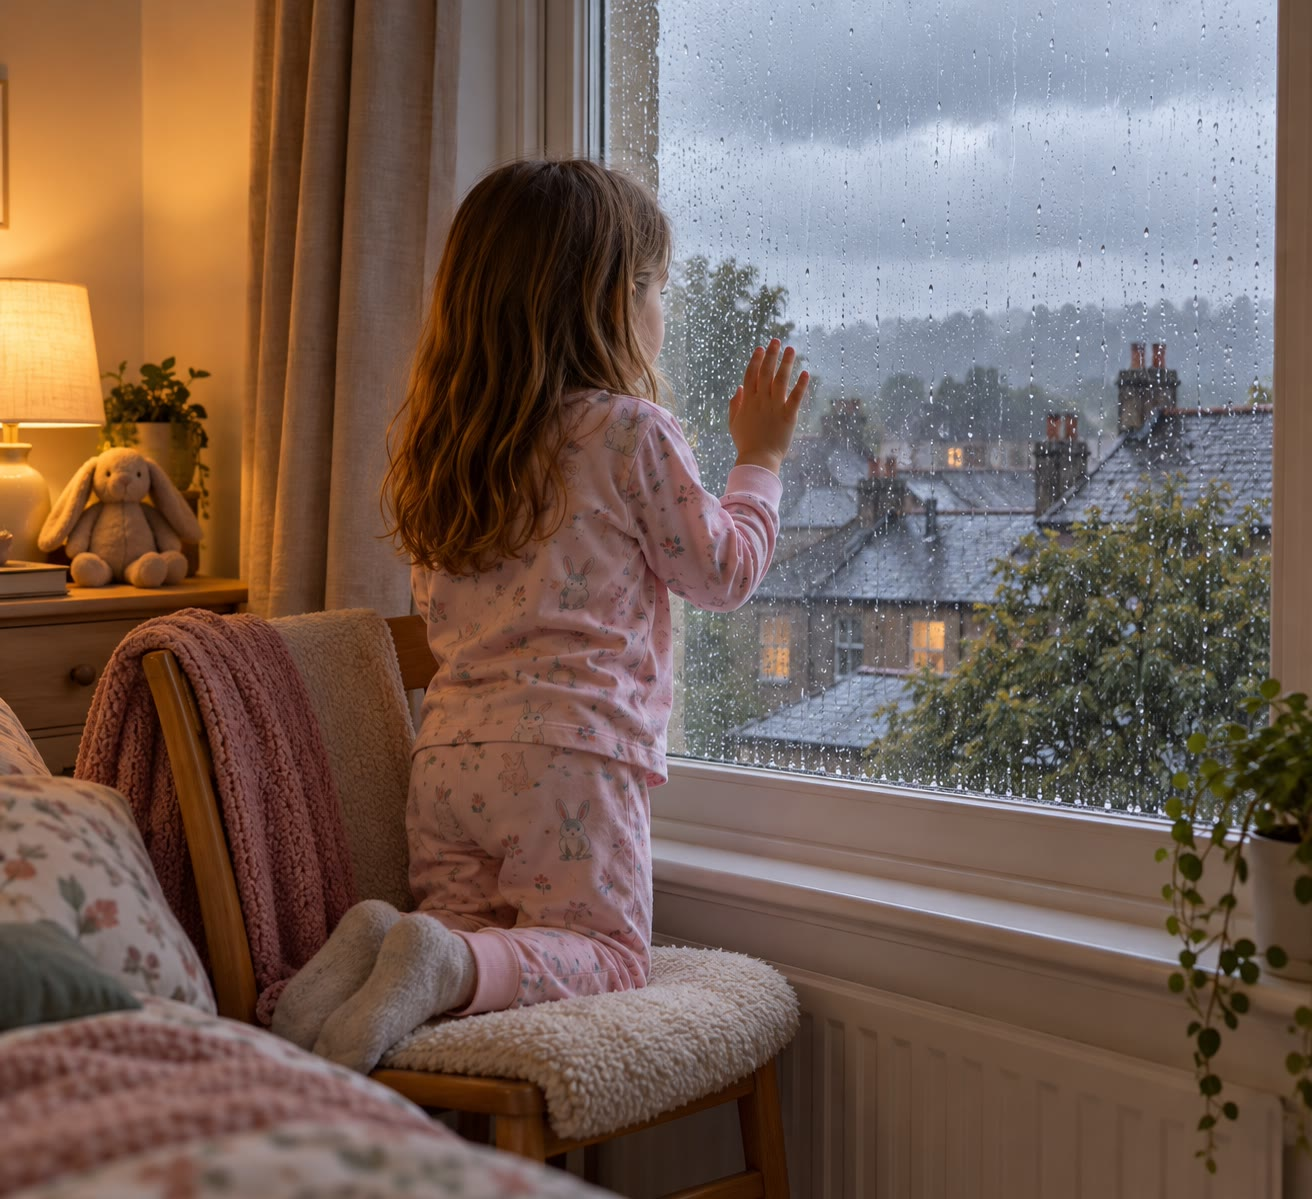
\includegraphics[width=0.72\linewidth]{images/book1/ai/g1-rainy-window.jpg}

{\small A grey, rainy morning seen through a window.}
\end{omfigure}

\begin{recall}
Every morning the Sun rises, and the day begins; every evening it sets, and
the night comes. In the physics books you have seen why day follows night.
In this chapter we look at something else that changes all the time: the
\omterm{def:g1:watching-the-weather:weather}{weather}.
\end{recall}

\section{What is the weather?}

When we go outside, we feel the air on our face. It may be warm or cold. It
may be still, or it may push our hair and our clothes: then there is wind.
We look up at the sky. It may be blue and bright, or covered with clouds.
Sometimes rain falls from the clouds, sometimes snow. All of this together
is the \omterm{def:g1:watching-the-weather:weather}{weather}.

\begin{definition}[Weather]\label{def:g1:watching-the-weather:weather}
The \emph{weather}\index{weather} is what the air and the sky are like in
one place at one moment: sunny or cloudy, dry or rainy or snowy, calm or
windy, warm or cold.
\end{definition}

To describe the \omterm{def:g1:watching-the-weather:weather}{weather}, we answer a few simple questions:
\begin{enumerate}
  \item \textbf{What does the sky look like?} Is it blue, with the Sun
        shining? Are there a few clouds, or is the sky all grey?
  \item \textbf{Is anything falling from the sky?} Rain? Snow? Nothing?
  \item \textbf{Is there wind?} Do the leaves of the trees move? Does a
        flag flap?
  \item \textbf{Is it warm or cold?} Do we need a coat?
\end{enumerate}

\begin{omfigure}
\begin{minipage}[b]{0.49\linewidth}\centering
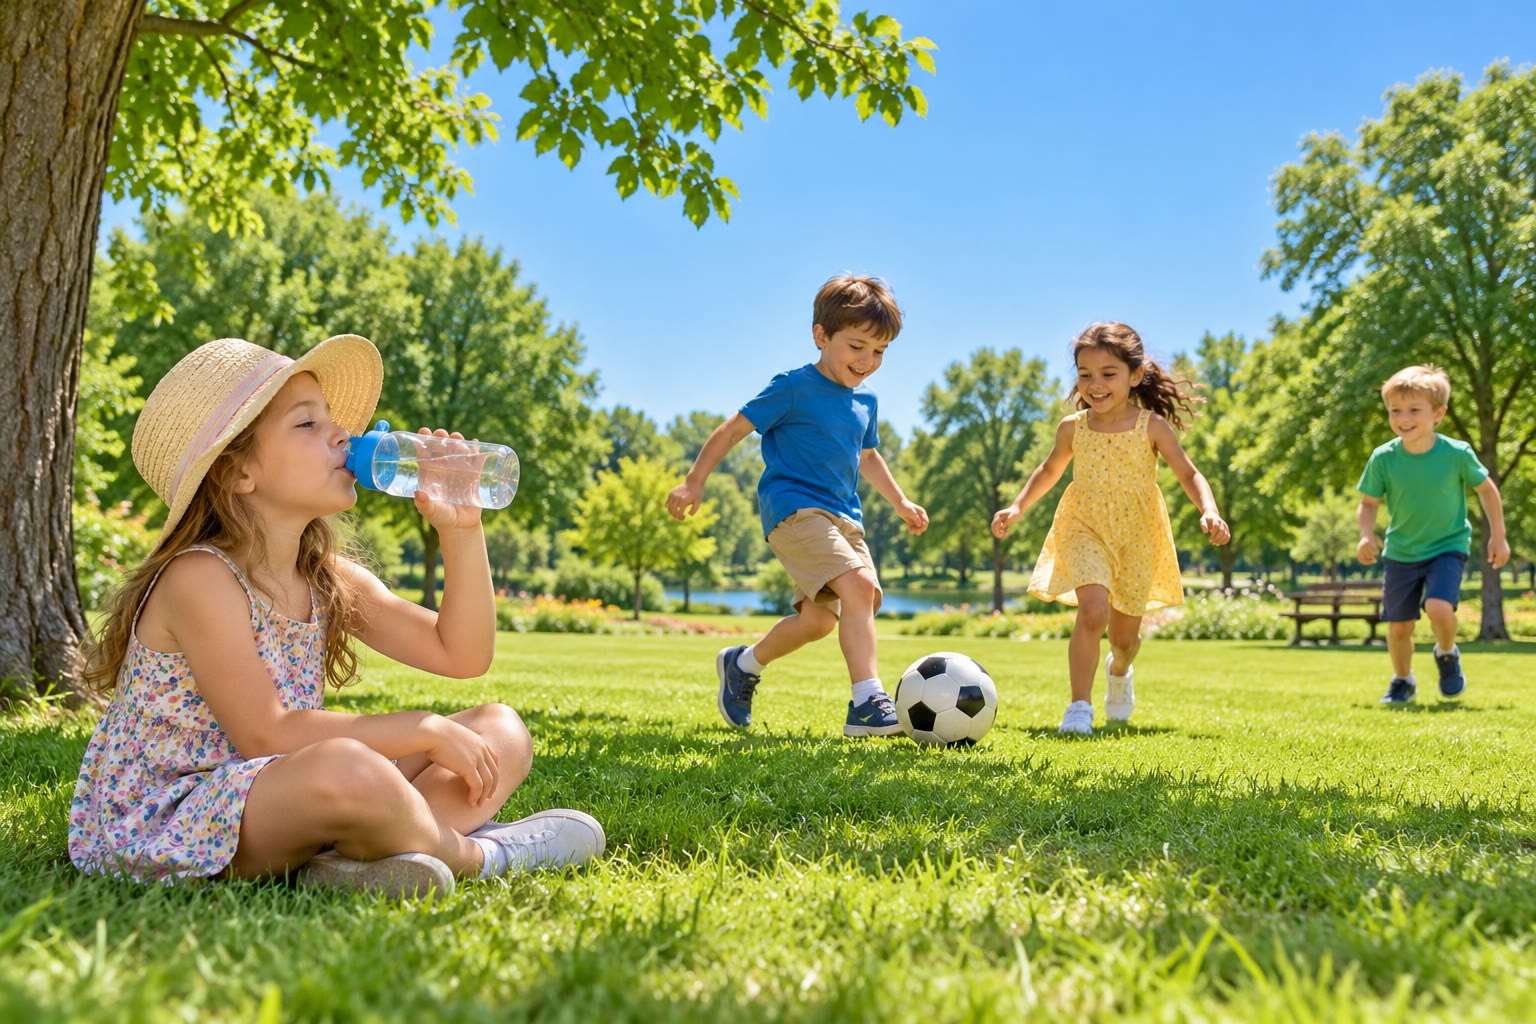
\includegraphics[width=\linewidth]{images/book1/ai/g1-sunny-park.jpg}

{\small Sunny and warm.}
\end{minipage}\hfill
\begin{minipage}[b]{0.49\linewidth}\centering
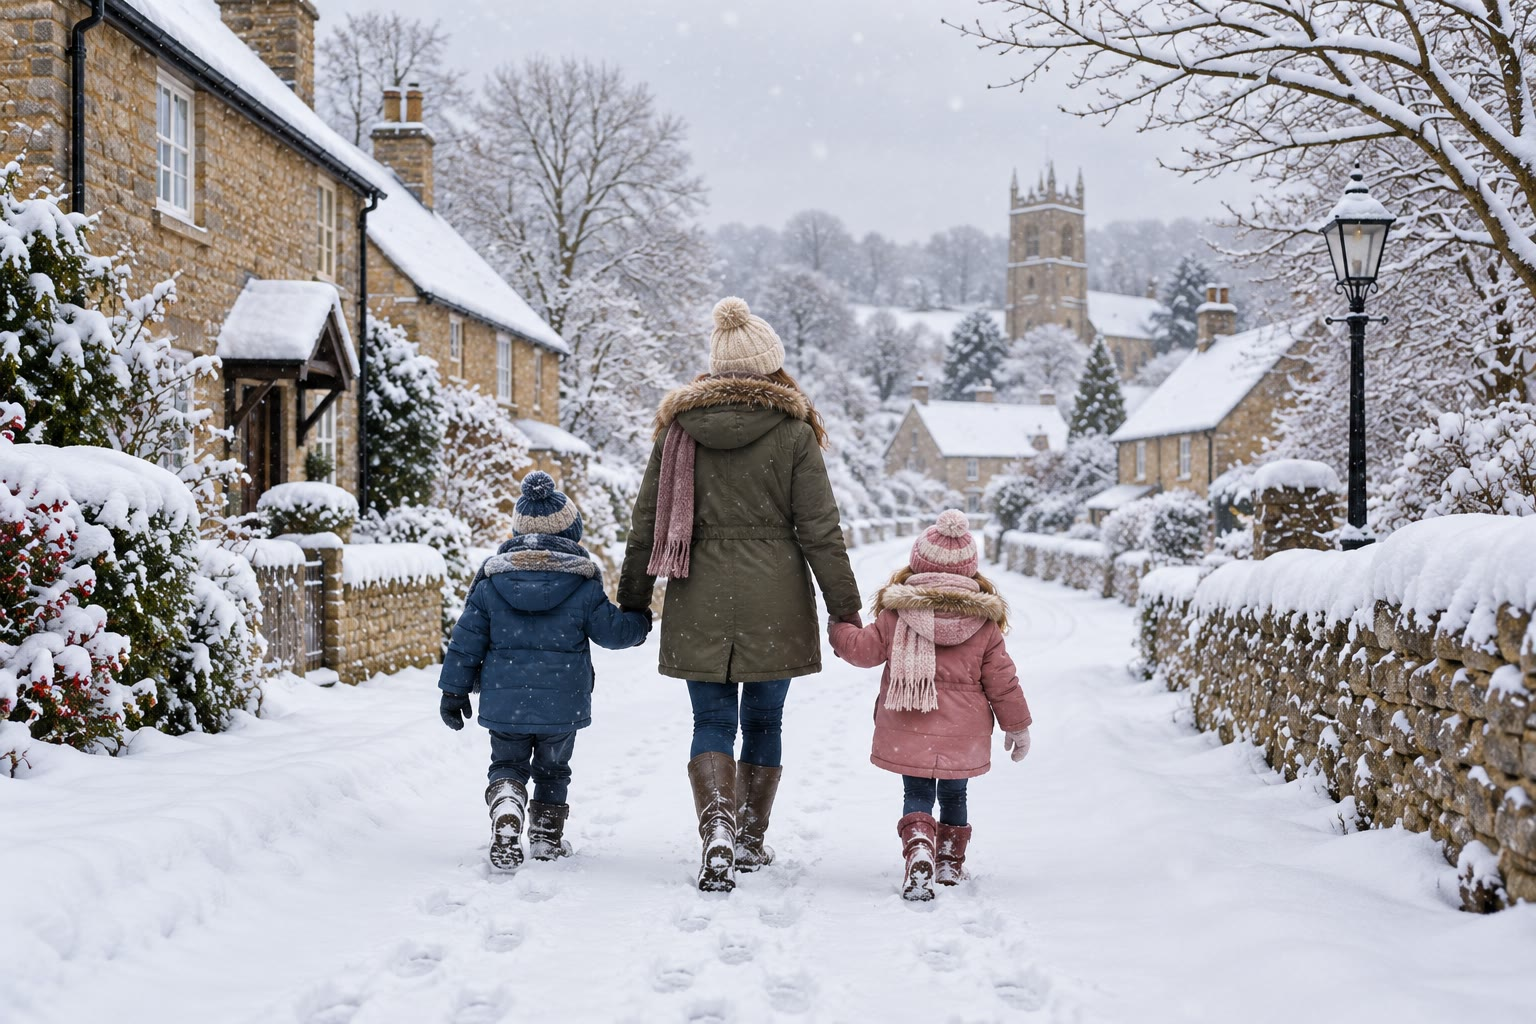
\includegraphics[width=\linewidth]{images/book1/ai/g1-snowy-street.jpg}

{\small Snowy and cold.}
\end{minipage}

\medskip
\begin{minipage}[b]{0.49\linewidth}\centering
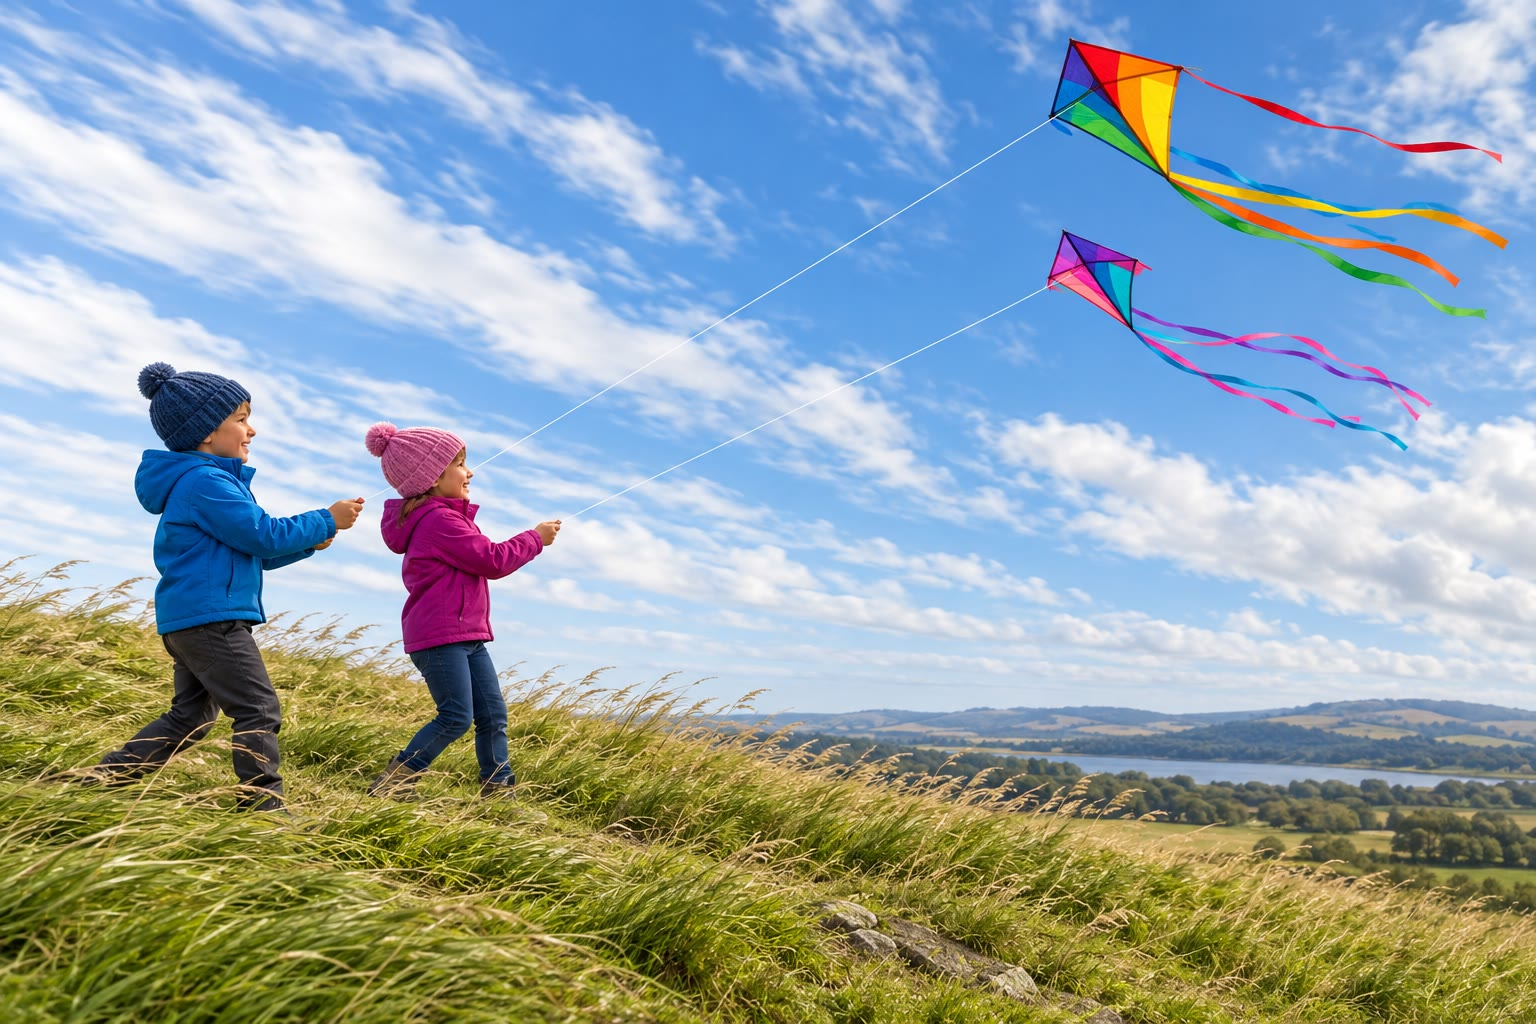
\includegraphics[width=\linewidth]{images/book1/ai/g1-windy-kites.jpg}

{\small Windy: the kites fly.}
\end{minipage}\hfill
\begin{minipage}[b]{0.49\linewidth}\centering
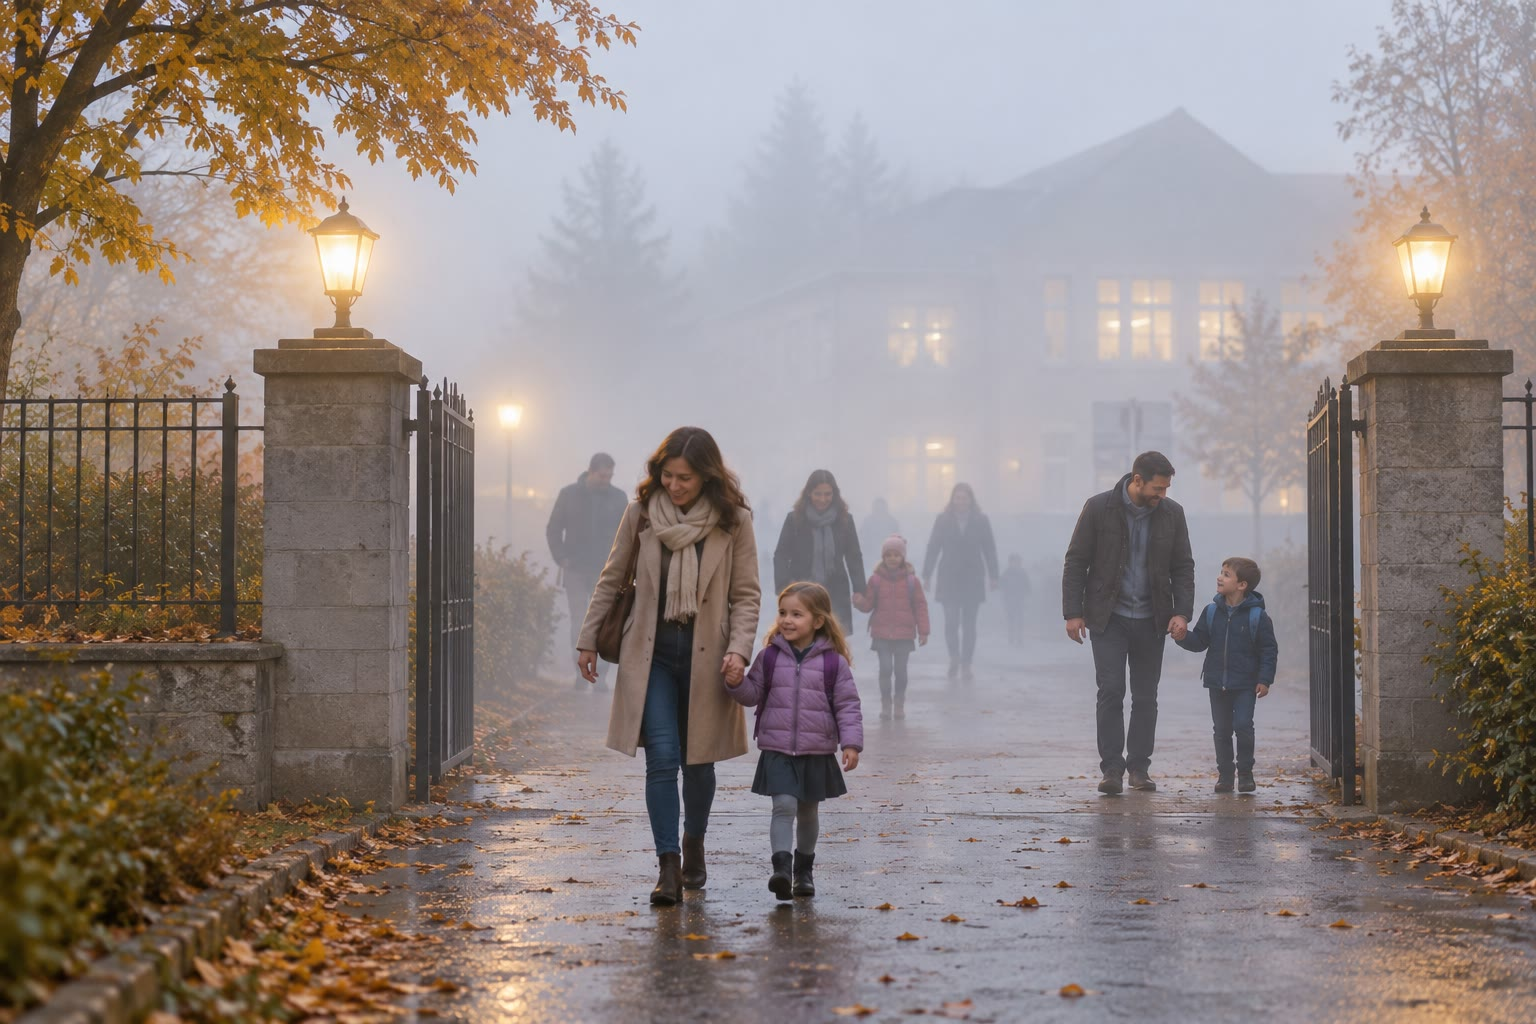
\includegraphics[width=\linewidth]{images/book1/ai/g1-foggy-school.jpg}

{\small Foggy: we cannot see far.}
\end{minipage}
\end{omfigure}

\begin{example}[Fog]\label{ex:g1:watching-the-weather:fog}
On some mornings the air itself looks white, and the trees at the end of
the street seem to disappear. This is fog. Fog is a cloud that touches the
ground. When the day warms up, the fog often goes away.
\end{example}

\section{Weather symbols and the weather chart}

Drawing the \omterm{def:g1:watching-the-weather:weather}{weather} with words takes a long time. People who watch the
\omterm{def:g1:watching-the-weather:weather}{weather} use small pictures instead: \omterm{def:g1:watching-the-weather:weather-chart}{weather symbols}. Each symbol is easy to
draw and easy to recognise.

\begin{omfigure}
\begin{tikzpicture}[x=1cm, y=1cm]
  \foreach \i/\n/\t in {0/sun/sunny, 1/suncloud/sun and clouds,
      2/cloud/cloudy, 3/rain/rainy, 4/shower/showers} {
    \pic[scale=1.25, transform shape] at (\i*2.6,0) {omwx=\n};
    \node[font=\small, align=center, text width=2.4cm] at (\i*2.6,-1.05) {\t};
  }
  \foreach \i/\n/\t in {0/snow/snowy, 1/storm/thunderstorm, 2/fog/foggy,
      3/wind/windy} {
    \pic[scale=1.25, transform shape] at (\i*2.6+1.3,-2.6) {omwx=\n};
    \node[font=\small, align=center, text width=2.4cm] at (\i*2.6+1.3,-3.65) {\t};
  }
\end{tikzpicture}

{\small Nine \omterm{def:g1:watching-the-weather:weather-chart}{weather symbols}. The thunderstorm has a dark cloud and a flash
of lightning; the showers come with sunny spells between them.}
\end{omfigure}

\begin{definition}[Weather chart]\label{def:g1:watching-the-weather:weather-chart}
A \emph{weather symbol}\index{weather symbol} is a small drawing that shows
one kind of \omterm{def:g1:watching-the-weather:weather}{weather}. A \emph{weather chart}\index{weather chart} is a table
in which we write down, day after day, the \omterm{def:g1:watching-the-weather:weather}{weather} we have seen, with
\omterm{def:g1:watching-the-weather:weather}{weather} symbols.
\end{definition}

A class can keep a \omterm{def:g1:watching-the-weather:weather-chart}{weather chart} for a whole week. Every morning, and again
every afternoon, one child looks outside and draws the symbol in the right
box. We also write whether it is warm or cold.

\begin{omfigure}
\begin{tikzpicture}[x=1cm, y=1cm]
  \def\cw{1.9}
  \foreach \d [count=\i from 0] in {Monday, Tuesday, Wednesday, Thursday,
      Friday, Saturday, Sunday}
    \node[font=\scriptsize\bfseries] at ({1.6+\i*\cw+\cw/2},0.35) {\d};
  \node[font=\scriptsize\bfseries, anchor=east] at (1.45,-0.5) {morning};
  \node[font=\scriptsize\bfseries, anchor=east] at (1.45,-1.5) {afternoon};
  \node[font=\scriptsize\bfseries, anchor=east, align=right] at (1.45,-2.35) {warm or\\cold?};
  \draw[black!60] (1.6,0) rectangle ({1.6+7*\cw},-2.7);
  \foreach \i in {1,...,6}
    \draw[black!60] ({1.6+\i*\cw},0.65) -- ({1.6+\i*\cw},-2.7);
  \draw[black!60] (1.6,0.65) -- ({1.6+7*\cw},0.65);
  \draw[black!60] (1.6,0.65) -- (1.6,0);
  \draw[black!60] ({1.6+7*\cw},0.65) -- ({1.6+7*\cw},0);
  \draw[black!60] (1.6,-1) -- ({1.6+7*\cw},-1);
  \draw[black!60] (1.6,-2) -- ({1.6+7*\cw},-2);
  \foreach \i/\m/\a/\w in {0/rain/rain/cold, 1/cloud/suncloud/cold,
      2/sun/sun/warm, 3/sun/suncloud/warm, 4/suncloud/shower/warm,
      5/fog/sun/warm, 6/cloud/rain/cold} {
    \pic[scale=0.8, transform shape] at ({1.6+\i*\cw+\cw/2},-0.5) {omwx=\m};
    \pic[scale=0.8, transform shape] at ({1.6+\i*\cw+\cw/2},-1.5) {omwx=\a};
    \node[font=\scriptsize] at ({1.6+\i*\cw+\cw/2},-2.35) {\w};
  }
\end{tikzpicture}

{\small The \omterm{def:g1:watching-the-weather:weather-chart}{weather chart} kept by a class for one week in spring.}
\label{fig:g1:watching-the-weather:chart}
\end{omfigure}

\begin{method}[Reading a weather chart]\label{met:g1:watching-the-weather:read}
To read a \omterm{def:g1:watching-the-weather:weather-chart}{weather chart}:
\begin{enumerate}
  \item find the column of the day you want;
  \item look at the row: morning, or afternoon;
  \item name the \omterm{def:g1:watching-the-weather:weather}{weather} that the symbol shows.
\end{enumerate}
To find how many days were sunny, run your finger along a row and count
the sun symbols.
\end{method}

\begin{example}[Reading the class chart]\label{ex:g1:watching-the-weather:read}
On the chart of this class, Monday morning was rainy and cold. On
Wednesday it was sunny all day. On Saturday a fog in the morning gave way
to sunshine in the afternoon. In the mornings of the week, the class drew
the sun on 2 days: Wednesday and Thursday.
\end{example}

\section{The weather changes}

The \omterm{def:g1:watching-the-weather:weather}{weather} does not stay the same. It changes during the day, from one day
to the next, and over the year.

\begin{itemize}
  \item \textbf{During one day.} A grey morning can turn into a sunny
        afternoon. A clear blue morning can end with a storm. In the early
        morning and at night it is usually cooler than in the afternoon.
  \item \textbf{From one day to the next.} Look at the class chart: no two
        days of the week are exactly the same.
  \item \textbf{Over the year.} In summer the days are usually warm, and in
        winter they are usually cold; in many places snow falls only in
        winter. The physics books explain why the seasons come back every
        year.
\end{itemize}

\begin{omfigure}
\begin{tikzpicture}[x=1cm, y=1cm]
  \draw[black!50, line width=0.8pt, -{Stealth[length=2.5mm]}] (0,0) -- (12.2,0);
  \foreach \x/\n/\t/\h in {0.9/fog/early morning/cool, 3.5/suncloud/morning/mild,
      6.1/sun/afternoon/warm, 8.7/storm/late afternoon/warm and stormy,
      11.2/suncloud/evening/cooler} {
    \pic[scale=1.1, transform shape] at (\x,0.85) {omwx=\n};
    \fill[black!60] (\x,0) circle (1.5pt);
    \node[font=\scriptsize\bfseries, below] at (\x,-0.12) {\t};
    \node[font=\scriptsize, below] at (\x,-0.5) {\h};
  }
\end{tikzpicture}

{\small One summer day, from the morning to the evening: the \omterm{def:g1:watching-the-weather:weather}{weather} changes
five times.}
\label{fig:g1:watching-the-weather:day}
\end{omfigure}

\begin{omfigure}
\begin{tikzpicture}[x=1cm, y=1cm]
  \foreach \i/\s/\c/\g/\w/\gr in {0/spring/green!55!black/pink!60/suncloud/green!35,
      1/summer/green!45!black/green!50!black/sun/green!35,
      2/autumn/orange!80!black/orange!70/rain/green!25!brown!30,
      3/winter/black!55/white/snow/white} {
    \begin{scope}[shift={(\i*3.15,0)}]
      \draw[black!30, rounded corners=3pt, fill=ocBlue!6] (-1.4,-0.45) rectangle (1.4,3.05);
      \fill[\gr] (-1.4,-0.45) rectangle (1.4,0);
      \draw[black!25] (-1.4,0) -- (1.4,0);
      \fill[brown!60!black] (-0.09,0) rectangle (0.09,1.0);
      \draw[brown!60!black, line width=1.6pt] (0,0.75) -- (-0.5,1.35);
      \draw[brown!60!black, line width=1.6pt] (0,0.9) -- (0.45,1.45);
      \ifnum\i<3
        \fill[\c, opacity=0.85] (0,1.55) circle (0.72);
        \ifnum\i=0 \foreach \a in {20,80,140,200,260,320} \fill[\g] (0,1.55) ++(\a:0.45) circle (0.09); \fi
        \ifnum\i=2 \foreach \x/\y in {-0.9/0.15,0.7/0.3,0.95/0.1} \fill[\g] (\x,\y) circle (0.07); \fi
      \else
        \draw[white, line width=2.4pt] (-0.5,1.35) -- (-0.35,1.17);
        \draw[white, line width=2.4pt] (0.45,1.45) -- (0.3,1.27);
      \fi
      \pic[scale=0.8, transform shape] at (0.95,2.55) {omwx=\w};
      \node[font=\small\bfseries] at (0,-0.75) {\s};
    \end{scope}
  }
\end{tikzpicture}

{\small The same tree in the four seasons: blossom in spring, thick green
leaves in summer, falling orange leaves in autumn, bare branches with snow
in winter.}
\label{fig:g1:watching-the-weather:seasons}
\end{omfigure}

\begin{remark}[Where the wind comes from]\label{rem:g1:watching-the-weather:wind}
We cannot see the wind, but we can see what it does. A flag, a windsock or
the smoke from a chimney is pushed by the wind: they point to where the
wind is going, so the wind comes from the other side.
\end{remark}

\begin{omfigure}
\begin{tikzpicture}[x=1cm, y=1cm]
  % ground
  \fill[green!30!omLithAlluv] (-0.4,-0.1) rectangle (8.4,0);
  % windsock on a pole
  \draw[black!70, line width=1.2pt] (1,0) -- (1,3.2);
  \fill[orange!85, draw=black!60] (1,3.15) -- (3.4,2.95) -- (3.4,2.55) -- (1,2.45) -- cycle;
  \fill[white] (1.6,3.1) -- (2.2,3.05) -- (2.2,2.5) -- (1.6,2.47) -- cycle;
  \fill[white] (2.8,3.0) -- (3.4,2.95) -- (3.4,2.55) -- (2.8,2.53) -- cycle;
  \draw[black!60] (1,3.15) -- (3.4,2.95) -- (3.4,2.55) -- (1,2.45);
  % flag
  \draw[black!70, line width=1.2pt] (5.4,0) -- (5.4,3.2);
  \fill[ocBlue!70, draw=black!60] (5.4,3.15) .. controls (6.0,3.3) and (6.4,2.9) .. (7.1,3.05)
     -- (7.1,2.35) .. controls (6.4,2.2) and (6.0,2.6) .. (5.4,2.45) -- cycle;
  % wind arrows
  \foreach \y in {1.0,1.6}
    \draw[omWxRain, line width=1.4pt, -{Stealth[length=3mm]}] (-0.3,\y) -- (0.7,\y);
  \node[font=\small, align=right, anchor=east] at (-0.45,1.3) {the wind\\comes from here};
  \draw[black!60, -{Stealth[length=2mm]}] (4.1,2.75) -- (4.9,2.75);
  \node[font=\small, align=left, anchor=west] at (7.5,2.7) {flag and windsock\\point where the\\wind is going};
\end{tikzpicture}

{\small A windsock and a flag on a windy day. The wind blows from the left
to the right.}
\end{omfigure}

\section{Why do we watch the weather?}

Many people need to know what the \omterm{def:g1:watching-the-weather:weather}{weather} will be like.
\begin{itemize}
  \item \textbf{Farmers} watch the sky before they cut the hay: rain would
        spoil it. In spring they fear a frosty night that could kill the
        young plants.
  \item \textbf{Sailors and fishermen} watch the wind: a strong wind makes
        big waves, and boats stay in the harbour.
  \item \textbf{Pilots} need to know about fog, storms and wind before an
        aeroplane takes off.
  \item \textbf{A class} that goes on an outing to the forest wants to know
        whether to take raincoats or sun hats.
\end{itemize}
Every day, people called meteorologists watch the \omterm{def:g1:watching-the-weather:weather}{weather} all over the
world and tell us, on the radio, on television or on a phone, what the
\omterm{def:g1:watching-the-weather:weather}{weather} will probably be like in the next days.

\begin{example}[Signs in the sky]\label{ex:g1:watching-the-weather:signs}
Long before radios and phones, people learnt to read the sky. When small
white clouds grow, in the afternoon, into tall dark towers, a shower or a
thunderstorm is coming. When the wind turns and the sky slowly fills with a
grey veil, rain often follows a few hours later. These signs are not always
right, but they are often useful.
\end{example}

\section{Dressing for the weather}

Now Lena can answer her question. It is raining and it is cold, so she will
wear her raincoat and her boots. Tomorrow the \omterm{def:g1:watching-the-weather:weather}{weather} may be different, and
she will choose again.

\begin{omfigure}
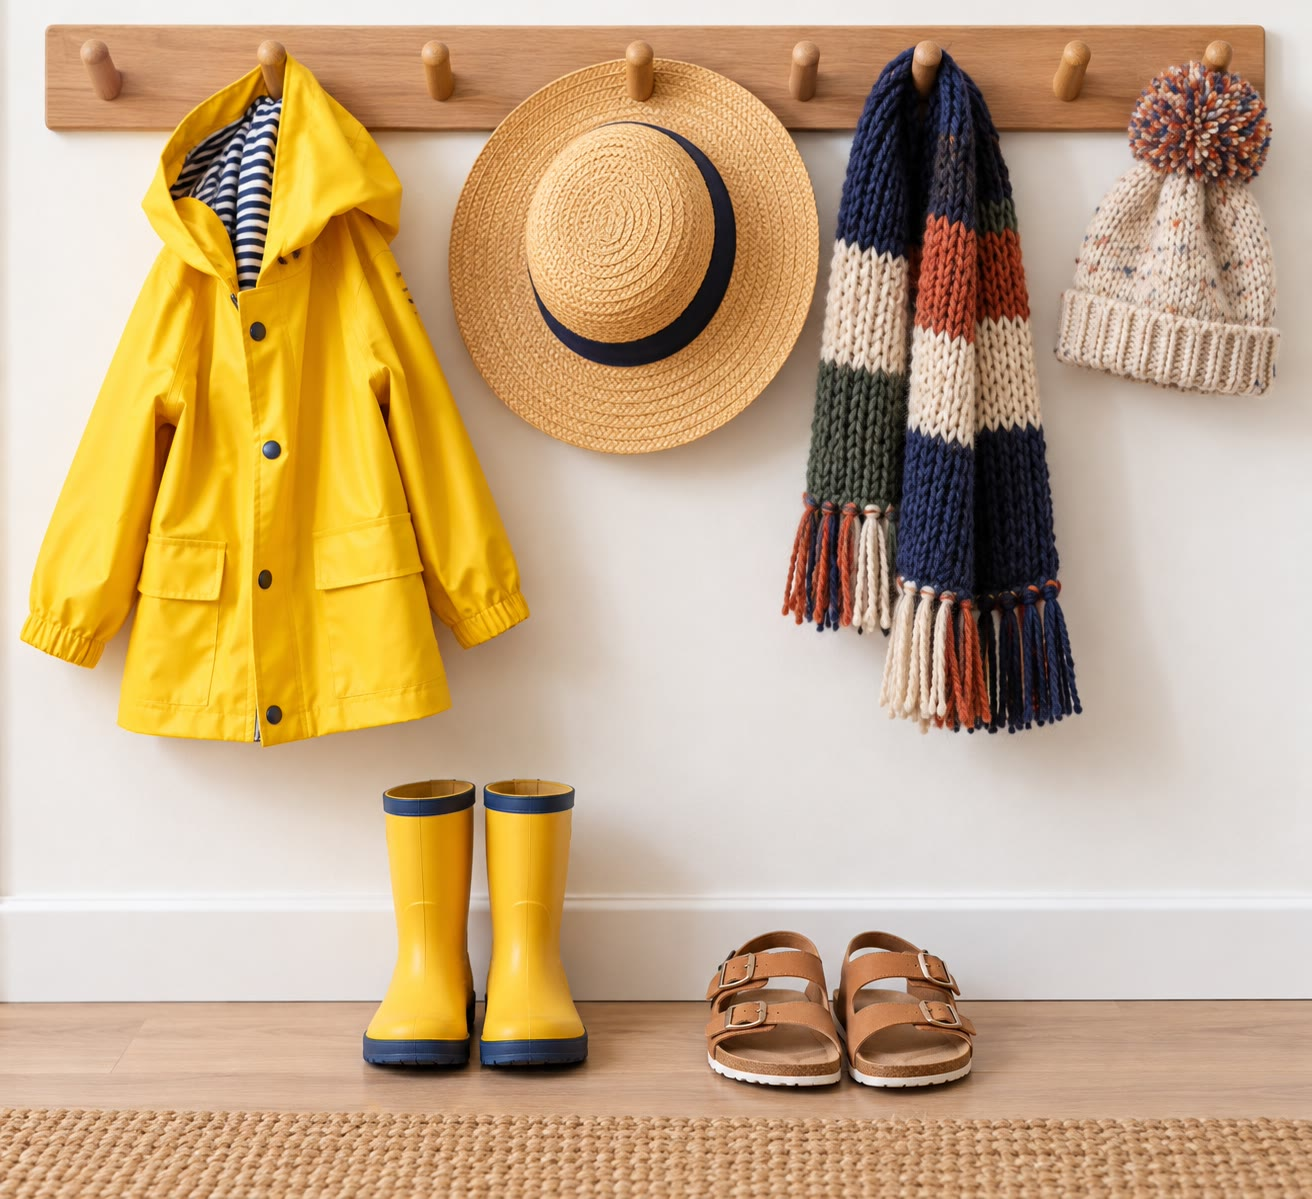
\includegraphics[width=0.66\linewidth]{images/book1/ai/g1-coat-pegs.jpg}

{\small Clothes for every kind of \omterm{def:g1:watching-the-weather:weather}{weather}: a raincoat, a sun hat, a scarf
and a warm hat, boots and sandals.}
\end{omfigure}

\begin{method}[Choosing clothes for the weather]\label{met:g1:watching-the-weather:clothes}
Look at the sky and feel the air, then:
\begin{itemize}
  \item rain or showers: a raincoat or an umbrella, and boots;
  \item cold or snow: a warm coat, a scarf, a hat and gloves;
  \item strong sunshine and heat: a sun hat, light clothes, and water to
        drink;
  \item wind: a coat that closes well; an umbrella is not much help.
\end{itemize}
\end{method}

\begin{safety}
\textbf{Never look straight at the Sun}, not even for a moment, and never
through glasses, binoculars or a camera: it can hurt your eyes for ever.
When there is a thunderstorm, stay indoors or in a car, keep away from tall
trees and from water, and wait until the storm has passed.
\end{safety}

\section{Exercises}

\begin{exercise}[$\star$]\label{exo:g1:watching-the-weather:1}
Draw the symbol for each kind of \omterm{def:g1:watching-the-weather:weather}{weather}: sunny; rainy; snowy; cloudy.
\end{exercise}

\begin{exercise}[$\star$]\label{exo:g1:watching-the-weather:2}
What is the \omterm{def:g1:watching-the-weather:weather}{weather} like in each of the four pictures of the section
``What is the \omterm{def:g1:watching-the-weather:weather}{weather}?''? Use one or two words for each.
\end{exercise}

\begin{exercise}[$\star$]\label{exo:g1:watching-the-weather:3}
Look at the class \omterm{def:g1:watching-the-weather:weather-chart}{weather chart}. What was the \omterm{def:g1:watching-the-weather:weather}{weather} on Tuesday morning?
On Friday afternoon? On Sunday afternoon?
\end{exercise}

\begin{exercise}[$\star$]\label{exo:g1:watching-the-weather:4}
On the class \omterm{def:g1:watching-the-weather:weather-chart}{weather chart}, on which day was it sunny in the morning and in
the afternoon?
\end{exercise}

\begin{exercise}[$\star$]\label{exo:g1:watching-the-weather:5}
Match each piece of clothing with a \omterm{def:g1:watching-the-weather:weather}{weather}: a sun hat; boots and a
raincoat; a scarf and gloves. The \omterm{def:g1:watching-the-weather:weather}{weathers} are: cold and snowy; hot and
sunny; rainy.
\end{exercise}

\begin{exercise}[$\star$]\label{exo:g1:watching-the-weather:6}
Lena says: ``Look, the flag is flapping!'' What kind of \omterm{def:g1:watching-the-weather:weather}{weather} is it?
\end{exercise}

\begin{exercise}[$\star$]\label{exo:g1:watching-the-weather:7}
True or false? Explain.
\begin{enumerate}
  \item The \omterm{def:g1:watching-the-weather:weather}{weather} is always the same in the morning and in the afternoon.
  \item Fog is a cloud that touches the ground.
  \item The rule ``never look at the Sun, not even with one eye'' is a good rule.
\end{enumerate}
\end{exercise}

\begin{exercise}[$\star\star$]\label{exo:g1:watching-the-weather:8}
On the class \omterm{def:g1:watching-the-weather:weather-chart}{weather chart}, count the afternoons with rain or showers.
Count the cold days. Was the week mostly warm or mostly cold?
\end{exercise}

\begin{exercise}[$\star\star$]\label{exo:g1:watching-the-weather:9}
Here is what Sam saw from his window during one day: in the morning, a grey
sky; at lunchtime, drops on the window; in the evening, a blue sky with a
few clouds. Draw the three \omterm{def:g1:watching-the-weather:weather-chart}{weather symbols} in the right order.
\end{exercise}

\begin{exercise}[$\star\star$]\label{exo:g1:watching-the-weather:10}
On the picture of the windsock and the flag, the wind comes from the left.
On another day, a flag points to the left. From which side does the wind
come that day?
\end{exercise}

\begin{exercise}[$\star\star$]\label{exo:g1:watching-the-weather:11}
Look at the drawing of the same tree in the four seasons. In which season
does the tree have no leaves? In which season does it have blossom? Which
\omterm{def:g1:watching-the-weather:weather-chart}{weather symbol} is drawn for winter, and why does it fit that season?
\end{exercise}
